\subsection{Measured successor results}
The two successor problems have 14 and 18 columns, distinct from the 8, 12, 16,
and 20-column performance problems. They follow the same synthetic construction
family; they do not establish transfer to a new industrial domain. Both exact
concentration distributions agree with the independently implemented conventional
semiring dynamic program.

\begin{table}[htbp]
\centering\small
\setlength{\tabcolsep}{4pt}
\begin{tabular}{@{}lrrrrr@{}}
\toprule
Problem & Fiber size & Warm & Cold & Fresh, all $K$ & Fresh, $K=0$\\
\midrule
$4\times 14$ & 418,474,536 & 0.0063 & 0.2831 & 0.2474 & 0.0035 \\
$4\times 18$ & 379,555,919,108 & 0.0830 & 2.2568 & 1.5193 & 0.0085 \\
\bottomrule
\end{tabular}
\caption{Executed successor count queries; times are local seconds. Warm evaluates
the retained graph. Cold adds read, parse, and validation. Fresh all-$K$ computes
the same complete distribution from the request. Fresh $K=0$ computes only that
target, using the binary-cap equivalence. The target column is a different,
narrower contract, not an all-statistics speed comparison.}
\label{tab:successor}
\end{table}

\begin{figure}[htbp]
\centering
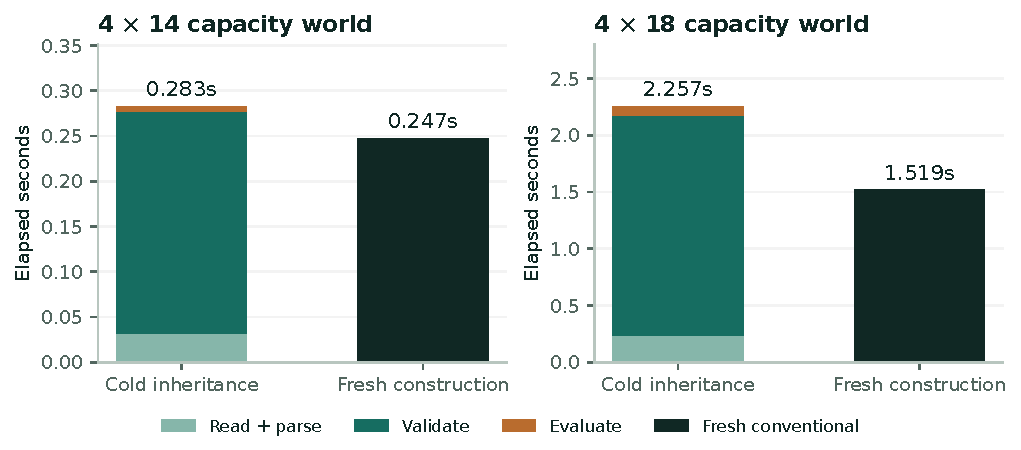
\includegraphics[width=\linewidth]{figures/successor_transfer.pdf}
\caption{Inheritance is useful in memory, but cold validation dominates these
transfers. Fresh conventional construction is faster for the same all-statistics
query on both held-out sizes. Predecessor construction and export are excluded
from these bars and reported separately below; adding them further increases
the full life-cycle cost of inheritance.}
\label{fig:successor}
\end{figure}

The 14-column asset has 504 states and 12,245 edges; the 18-column asset has
1,316 states and 76,943 edges. Their serialized JSON sizes are 1,339,844 and
8,512,360 bytes, compressed to 87,169 and 577,818 bytes. Predecessor construction
takes 0.1238 and 0.9237 seconds; export takes a further 0.1885 and 1.1112 seconds.
These costs are paid before the cold-query measurements. The complete construction,
export, and cold-query paths therefore take approximately 0.5954 and 4.2917 seconds.
No remote-network transfer or multi-year storage cost was measured.

\begin{table}[htbp]
\centering\small
\begin{tabular}{@{}lrrrr@{}}
\toprule
Problem & $K$ & Exact conditioned count & Generation seconds & Accepted tables\\
\midrule
$4\times 14$ & 0 & 94,968 & 0.0177 & 100 \\
$4\times 14$ & 1 & 996,336 & 0.0183 & 100 \\
$4\times 18$ & 0 & 5,444,610 & 0.0650 & 100 \\
$4\times 18$ & 1 & 78,007,280 & 0.0698 & 100 \\
\bottomrule
\end{tabular}
\caption{Fresh conditioned outputs generated from the inherited instrument.
Generation time is additional to obtaining the distribution and loading the asset.
Each of the 400 saved tables passes the original margins, caps, and requested
concentration check. These are computational acceptances, not customer acceptances.}
\end{table}

At 18 columns, only about $1.43\times10^{-5}$ of the uniform fiber has $K=0$.
That makes blind rejection unattractive, but the exact binary-cap simplification
computes its count in 0.0085 seconds. The separate target-specific comparator
measures counting, not generation of 100 outputs; no sample-generation speedup
over that comparator is asserted. The all-statistics comparison has the same
output contract on both sides.

The equal-inheritance control gives a conventional caller the same code and
artifact and obtains identical seeded conditioned outputs (20 at $K=1$ per
problem). This is an asset-availability control, not a second independent
implementation. It rejects exclusive ownership of the reuse benefit. The
independent full-distribution implementation supplies the separate numerical
correctness challenge.

\begin{evidencebox}
\textbf{Successor disposition.} Four hundred accepted conditioned worlds are
new outputs, and the instrument supplies a working productive inheritance.
The measured cold cost exceeds fresh conventional construction in both cases,
and conventional access to the same asset matches the result. Superior
transferred capability, an AI-specific advantage, and economically self-financing
succession are not established.
\end{evidencebox}
